







   If the area of $\triangle ACD$ is 100 and $B$ is the midpoint of $\overline{AC}$, then what is the $(x,y)$ coordinate of $B$?

\begin{center}
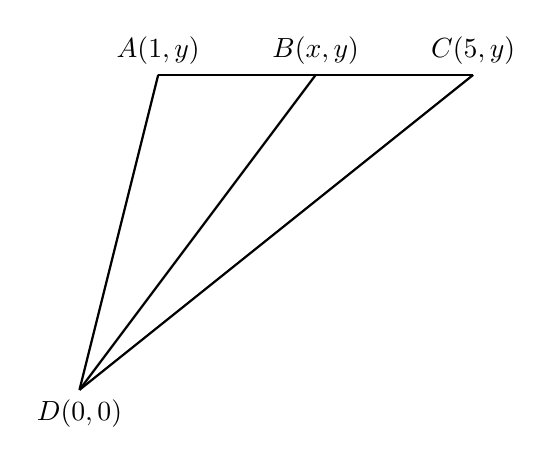
\begin{tikzpicture}
    \draw[thick] (0,0)--(1,4) node[above]{$A(1,y)$};              
    \draw[thick] (1,4)--(5,4) node[above]{$C(5,y)$}; 
    \draw[thick] (0,0)--(3,4) node[above]{$B(x,y)$};
    \draw[thick] (5,4)--(0,0) node[below]{$D(0,0)$};
\end{tikzpicture}
\end{center}



\ifsat
	\begin{enumerate}[label=\Alph*)]
		\item  $(2.5,50)$
		\item  $(2.5,25)$
		\item  $(3,50)$ %
		\item  $(3,25)$ 
	\end{enumerate}
\else
\fi

\ifacteven
	\begin{enumerate}[label=\textbf{\Alph*.},itemsep=\fill,align=left]
		\setcounter{enumii}{5}
		\item  $(2.5,50)$
		\item  $(2.5,25)$
		\item  $(3,50)$ %
		\addtocounter{enumii}{1}
		\item  $(3,25)$ 
		\item  $(3,30)$ 
	\end{enumerate}
\else
\fi

\ifactodd
	\begin{enumerate}[label=\textbf{\Alph*.},itemsep=\fill,align=left]
		\item  $(2.5,50)$
		\item  $(2.5,25)$
		\item  $(3,50)$ %
		\item  $(3,25)$ 
		\item  $(3,30)$ 
	\end{enumerate}
\else
\fi

\ifgridin
  $(3,50)$ %
		
\else
\fi

